% !TEX root = morphkasten.tex


%##############
\subsection{Farbsensor}
\begin{figure}[h]
	\centering
	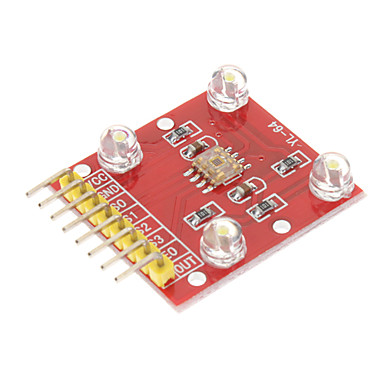
\includegraphics[width=0.5\textwidth]{fig/Farbsensor}
	\caption{Freedomboard KL25 von Freescale (Quelle: www.miniinthebox.com)}
	%http://miniimg1.rightinthebox.com/images/384x384/201310/bvlklo1383018315288.jpg
\end{figure}


\begin{table}[h]
\begin{tabular}{p{0.5\textwidth} | p{0.5\textwidth}}


 \textbf{Vorteile} & \textbf{Nachteile} \\ \hline
	 
\begin{itemize}
\item Im Preisrahmen, ein Farbsensor kostet ungefähr 10.-
\end{itemize}

 &
 
\begin{itemize}
\item Benötigt  AD Eingänge
\item Distanz abhängig
\end{itemize}

\end{tabular}
\end{table}

\begin{table}[h]
\begin{tabular}{p{0.5\textwidth}p{0.5\textwidth}}


 \textbf{Risiken} & \\ \hline
	 
\begin{itemize}
\item Distanz hat zu grossen Einfluss auf die Farberkennung
\item Die Farben lassen sich nicht zuverlässig erkennen (Sensorseite)
\end{itemize}
&
\begin{itemize}
\item Die Auswertung ist sehr aufwändig (Mikrocontrollerseitig)
\end{itemize}

 
\end{tabular}
\end{table}

\pagebreak


%##############
\subsection{Ultraschallsensoren}
\begin{figure}[h]
	\centering
	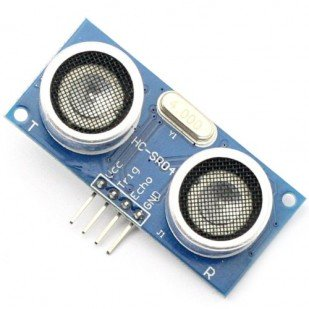
\includegraphics[width=0.5\textwidth]{fig/ultraschallsensor.png}
	\caption{Beispielhaftes Tinkerforge System (Bricks mit Ultraschallmodul) (Quelle: www.generationrobots.com)}
	%http://www.generationrobots.com/2653-large_default/ultraschallsensor-hc-sr04.jpg
\end{figure}

\begin{table}[h]
\begin{tabular}{p{0.5\textwidth} | p{0.5\textwidth}}


\textbf{Vorteile} & \textbf{Nachteile} \\ \hline
	 
\begin{itemize}
\item Erschwinglich, ein Sensor kostet ungefähr 5.Fr
\item Unempfindlich auf Störeinflüsse (Ausser andere Ultraschallsensoren)
\item Grosse Distanz (>10cm)
\end{itemize}
 &
\begin{itemize}
\item Kann nicht als als Liniensensor eingesetzt werden
\item Keine klaren Grenzen (relativ grosser Abstrahlwinkel)
\end{itemize}
\end{tabular}
\end{table}


\begin{table}[h]
\begin{tabular}{p{0.5\textwidth}p{0.5\textwidth}}


 \textbf{Risiken} & \\ \hline
	 
\begin{itemize}
\item Andere Ultraschallsensoren stören die Messung
\item Der Bereich ist zu ungenau
\end{itemize}
&
\begin{itemize}
\item Die Anbindung funktioniert nicht richtig
\end{itemize}

 
\end{tabular}
\end{table}

\pagebreak

%##############
\subsection{Infrarotsensoren}
\begin{figure}[h]
	\centering
	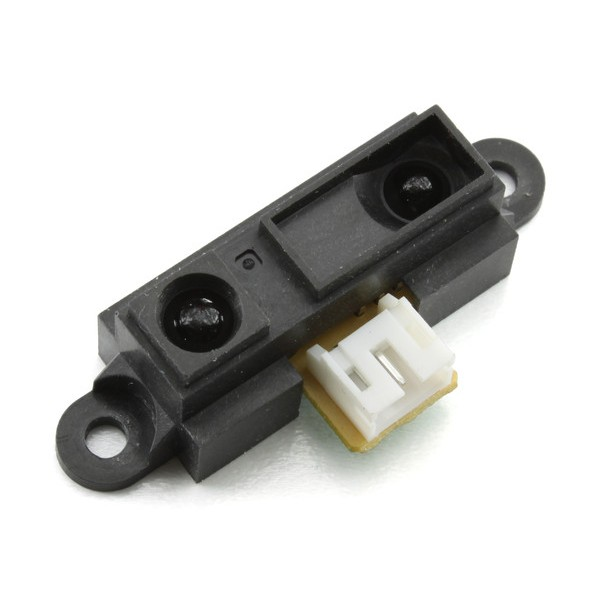
\includegraphics[width=0.5\textwidth]{fig/Infrarotsensor.jpg}
	\caption{Infrarotsensor (Quelle: www.tinkerforge.com)}
	%https://www.tinkerforge.com/de/shop/media/catalog/product/cache/2/image/600x600/9df78eab33525d08d6e5fb8d27136e95/s/e/sensor_gp2y0a21yk0f_tilted_600.jpg
\end{figure}

\begin{table}[h]
\begin{tabular}{p{0.5\textwidth} | p{0.5\textwidth}}


\textbf{Vorteile} & \textbf{Nachteile} \\ \hline
	 
\begin{itemize}
\item Kostengünstig (Sensor und Empfänger kosten zusammen 1.7Fr)
\item Kann als Liniensensor und Rad-Encoder eingesetzt werden.
\item Eher klaren Grenzen (kleiner Abstrahlwinkel)
\end{itemize}
 &
\begin{itemize}
\item Benötigt zwei AD Eingänge
\item Sind empfindlich auf UV-Licht
\item Geringe Reichweite (je nach Typ nur bis 5mm)
\item Als Liniensensor: Nicht senkrechtes Abtasten ist problematisch
\end{itemize}
\end{tabular}
\end{table}


\begin{table}[h]
\begin{tabular}{p{0.5\textwidth}p{0.5\textwidth}}


 \textbf{Risiken} & \\ \hline
	 
\begin{itemize}
\item Die Sensoren werden gestört
\item Die Sensoren sind zu ungenau
\end{itemize}
&
\begin{itemize}
\item Die Anbindung funktioniert nicht richtig
\end{itemize}

 
\end{tabular}
\end{table}

\pagebreak